\documentclass{article}  % list options between brackets
\usepackage{amsmath}              % list packages between braces
\usepackage[pdftex]{graphicx}
\usepackage{algorithm2e}

% type user-defined commands here

\begin{document}

\title{Application of machine learning algorithms for detection of cognitive impairment }   % type title between braces
\author{Robert Chen}         % type author(s) between braces
\date{March 10, 2010}    % type date between braces
\maketitle

\begin{abstract}
A major goal in Alzheimers disease research is to improve diagnostic tools. 
Currently, the Visual Paired Cognition (VPC) test is being used. Prior work in the lab has focused on using machine learning methods to serve as predictive tools for Alzheimers disease status using data from the VPC test. Different features of the VPC output have been implemented so far: pupil diameter, fixation duration, and novelty preference have been used in machine learning classifiers for the training stage.  The classification models would subsequently predict the case-control status of a given individual with a set of features. 

The main objective of the study is to improve the machine learning test by implementing new features into the model. For each of the images displayed in the VPC task, we calculated statistics for the visual saliency. We then normalized several features using the saliency statistics, and ran the classification algorithms with the normalized features. The results are reported in terms of accuracy and AUC statistics. 

In addition to machine learinng using the logistic regression classifier, we implemented classification using the hidden conditional random field (HCRF) and latent-dynamic discriminative conditional random field (LDCRF) models.

\end{abstract}

\section{Introduction}
Alzheimer's disease effects an estimated 5.4 million people and represents \$183 billion in annual costs. [\ref{ref:alz.org}]

\section{Methods}        

\subsection{Experimental Data -- Participants}
Data was collected from a previous study conducted by Lagun et al. (2011) in which subjects underwent the visual paired cognition test. The same subjects from the study conducted by Lagun et al. (2011) [\ref{ref:alz.org}] were used in this study. The subject groups consisted of (1) normal controls group (NC) consisting of 30 subjects without cognitive impairment; (2) Alzheimers disease group (AD) consisting of 20 subjects diagnosed with Alzheimers disease based on clinical criteria; and (3) mild cognitive impairment group (MCI) consisting of 10 subjects diagnosed based on clinical critieria.

\subsection{Experimental design -- VPC task setup}
See Lagun et al. (2011) for details on the VPC task setup.

\subsection{Data processing}
Various features were extracted from the data. For the features that were used in the study by Lagun et al. (2011), the features were extracted in the similar manner. These features are novelty preference (NP), vertical saccade orientation ($SO_v$), and fixation duration (FD). For this study, the NP, $SO_v$, and FD features for each given stage were normalized by the saliency metric (see later section for algorithm) 


\subsection{Machine learning for prediction of subject status}

\subsubsection{Logistic Regression}
We fit the subjects in the training set to a logistic regression model. Subsequently we predicted the cognitive status for the subjects using the features for these subjects. 

\paragraph{Cross-validation: logistic regression}
We used 3-fold and 5-fold cross-validation for the logistic regression classifier. For both of these situations, we repeated the cross-validation for 1000 iterations and reported the mean prediction accuracy statistics across all 1000 iterations. We performed 10-fold cross-validation as well but we noticed a steep drop off in accuracy in comparison to the 3-fold and 5-fold cross validation techniques. The cross validation is described in Algorithm \ref{algo:cv_logistic})


\begin{algorithm}{\textbf{Algorithm - Cross validation}}{
    \label{algo:cv_logistic}
}
\SetKwData{trainingGroup}{trainingGroup}
\SetKwData{testingGroup}{testingGroup}
\SetKwData{NC}{NC}
\SetKwData{MCI}{MCI}
\SetKwData{AD}{AD}
\SetKwData{NCtrain}{NCtrain}
\SetKwData{NCtest}{NCtest}
\SetKwData{results}{results}
\SetKwFunction{RunClassifier}{RunClassifier}


\Blankline\;
\For(\tcp*[f]{where $n$ is number of iterations}){$i = 1:1:n$}
{
\NCtrain $\leftarrow \frac{k-1}{k}(30)$ randomly chosen NC subjects\;
\trainingGroup $\leftarrow $ \AD $\cup$ \NCtrain \tcp*[f]{contains all AD subjects}\label{cmt}\;
\NCtest $\leftarrow \frac{1}{k}(30)$ randomly chosen NC subjects\;
\testingGroup  $\leftarrow $ \AD $\cup$ \NCtest \tcp*[f]{contains all MCI subjects}\label{cmt}\;
\results($i$) $\leftarrow$ \RunLogisticRegressionClassifier (\trainingGroup, \testingGroup)\;
}
%}%end of for loop
\Blankline
\caption{Cross validation for logistic regression classifier}
\end{algorithm}


%\paragraph{Algorithm - Logistic regression classifier}
\begin{algorithm}{\textbf{Algorithm - Logistic Regression classifier}}{
    \label{algo:logistic}}
\;
\tcp{Training:}\;
\Indp\Indp 
1. Initialize weights $w_m = 0$\;
2. Estimate log-odds ratio $w_m$ using maximum likelihood estimation\;
$w_m =$ argmax $l(w)$ \\
\Indp
where $l(w) = \sum_{i=1}^{n} (y_i log p(x_i, w) + \frac{(1-y_i)}{2} log (1 - p(x,w))$\\
and $p(x,w) = Pr(Y = 0, X = x) = \frac{1}{1 + exp(-(x^T w))}$ \;
\Indm
\Indm\Indm
\tcp{Testing:}
\Indp\Indp
1. estimate $Pr(Y = -1 | X = x)$ \\
\Indp\Indp where $p(x,w)  = \frac{1}{1 + e^{-(x^T w_m)}} $\;
\Indm\Indm 
2. Predict y=\left\{
\begin{array}{c l}      
    -1, & $Pr(Y = -1 | X=x)$ > $ Pr(Y=1 | X=x)$\\
    +1, & otherwise
\end{array}\right.

\Indm\Indm
\Blankline
\caption{Logistic regression classifier}
\end{algorithm}


\subsubsection{Conditional Random Field}
For each iteration, the 20 AD subjects were kept in the training set and the 10 MCI subjects were kept in the testing set. Of 30 MCI subjects, 20 are randomly assigned to the training set and the other 10 are applied to the testing set. Therefore, the training set consists of 40 total subjects and the testing set consists of 20 total subjects.

\paragraph{LDCRF model} 
The training set was trained with latent-dynamic conditional random field model, with subsequent classification of the testing set subjects (see figure \ref{fig:crfModels}). Four hidden states were used. Optimization with limited-memory BFGS algorithm (L-BFGS) was used in computing the model.

\paragraph{HCRF model}
The training set was trained with hidden conditional random field model, with subsequent classification of the testing set subjects  (see figure \ref{fig:crfModels}). Four hidden states were used. Optimization with limited-memory BFGS algorithm (L-BFGS) was used in computing the model.



\begin{figure}[htbp]
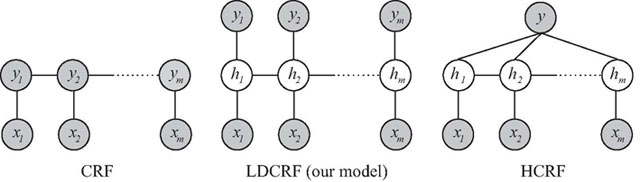
\includegraphics{crf_models.jpg}
\caption{Conditional random field, latent-dynamic discriminative conditional random field, and hidden conditional random field models.}
\label{fig:crfModels}
\end{figure}

\section{Results}









%%%%%%%%%%%%%%%%%%%%%%%%%%%%%%%%%%%%%%%%%%%%%%%%%%%%%%%%%%%%%%%%%%%%%%%
%%%%%%%%%%%%%%%%%%%%%%%%%%%%%%%



%%%%%%%%%%%%%%%%%%%%%%%%%%FIGURES

%\begin{figure}[htbp]
%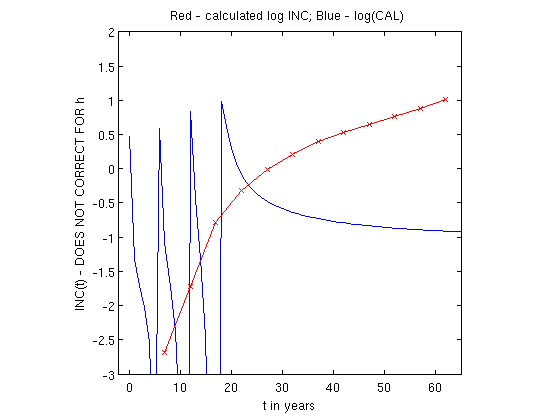
\includegraphics{CAL_inc_with_values_from_Kini.png}
%\caption{comparing calculated CAL vs INC}
%\label{fig:CAL_realINC_plot}
%\end{figure}



\end{document}
%
\begin{thebibliography}{9}
%  % type bibliography here
%{ref:alz.org} http://www.alz.org/downloads/Facts_Figures_2011.pdf
\end{thebibliography}


